\section{はじめに}
本章では、画像生成の仕組みについて解説します。高校数学の知識があれば理解できる範囲にとどめており、その上でAIを学ぶ楽しさを感じていただくことを目的としています。

AIを学ぶ醍醐味は大きく2つあります。1つ目が、広く利用されているものの、仕組みが不透明なAIについて学び、仕組みの不透明さを解消することで、AIが得体の知れないものから身近で理解可能な技術として捉えられるようになる点です。2つ目が、古典的なモデルから最新のモデルを順に学ぶことで、研究者たちの工夫やそれによる性能向上の歴史を追体験するような楽しみがある点です。

本章では、まず第2節でニューラルネットワークを画像データに適用できるように拡張した畳み込みニューラルネットワーク(CNN)について解説します。続いて、第3節では最も基本的な画像生成モデルであるオートエンコーダーを取り上げ、第4節および第5節では現在主流となっている拡散モデルおよび潜在拡散モデルについて解説します。
\section{畳み込みニューラルネットワーク(CNN)}
\subsection{畳み込みニューラルネットワークの概要}
前のページで紹介したニューラルネットワークでは、入力データを1次元配列として扱っていました。このような構造では、縦と横の空間的なつながりを持つ2次元画像データをうまく処理できません。そのため、画像の局所的特徴を捉えることができる\textgt{畳み込みニューラルネットワーク(CNN)}が使用されます。代表的なタスクとしては、0から9までの手書き数字画像を識別するもの(\textgt{MNISTデータセット})があります。図1は、MNISTデータセットの例です。
\begin{figure}[h]
\includegraphics[width=7cm]{image-gen/picture/kaishi0.pdf}
\centering
\caption{MNISTデータセット 出典:https://arxiv.org/pdf/2201.03898}
\end{figure}

畳み込みニューラルネットワークの起源は、1979年に計算機科学者の福島邦彦によって提唱されたネオコグニトロンにさかのぼります。これは、生物の脳の視覚野における情報処理の仕組みをモデル化したもので、現在のCNNの原型となりました。
\subsection{画像データの扱い方}
画像データは、各画素(ピクセル)の色を1つの要素とする2次元配列として扱われます。1画素の色は、光の三原色である赤(Red)、緑(Green)、青(Blue)の3成分で表現され、それぞれの成分の強さを0から1の範囲の実数値で表します。したがって、画像の解像度が縦$n$ピクセル、横$m$ピクセルの場合、画像データは$n \times m \times 3$の配列として表され、各要素は0から1の値をとるデータとして扱われます。画像データや、それに畳み込み処理を施して得られる2次元配列は、\textgt{特徴マップ}と呼ばれます。
\subsection{畳み込みニューラルネットワーク}
\begin{figure}[h]
\includegraphics[width=11cm]{image-gen/picture/kaishi1.pdf}
\centering
\caption{CNNの演算の様子 出典:https://arxiv.org/pdf/1603.07285}
\end{figure}
\begin{figure}[h]
\includegraphics[width=3cm]{image-gen/picture/kaishi2.pdf}
\centering
\caption{図1に適用したフィルタ 出典:https://arxiv.org/pdf/1603.07285}
\end{figure}
図2は、特徴マップに対して図3のフィルタを適用する様子を示します。具体的には、特徴マップの一部(図2では$3\times3$の領域)の左上から順にフィルタを重ね、フィルタの各要素と特徴マップの対応する要素を乗算し、それらの積の総和を求めるという処理を行います。図2の左上における計算は、次のように表されます。
\[
3\times0+3\times1+2\times2+0\times2+0\times2+1\times0+3\times0+1\times1+2\times2=12
\]

それぞれの特徴マップの一部にフィルタを適用するとき、フィルタを移動させる際の間隔(ピクセル数)を\textgt{ストライド(Stride)}と呼びます。図2の処理ではストライドは1となり、ストライドを2に設定すると、フィルタが2ピクセルずつ移動します。その結果、出力される特徴マップの縦横のサイズは約1/2になります。

このようにして、フィルタを画像全体に順に適用し、各位置で得られた値を並べることで、新しい特徴マップが得られます。

また、実際の画像データは、光の三原色である赤(Red)、緑(Green)、青(Blue)の各成分を表す2次元配列が3枚重なった構造をしています。これら3枚の画像データそれぞれに対して、複数種類のフィルタを適用することで、より多様な特徴を抽出することが可能です。図4は、3種類のフィルタを適用する様子を示しています。

\begin{figure}[h]
\includegraphics[width=7cm]{image-gen/picture/kaishi3.pdf}
\centering
\caption{複数種類のフィルタを適用 出典:https://arxiv.org/pdf/1603.07285}
\end{figure}

最後に、ReLUなどの活性化関数を通すことで、ニューラルネットワークの1層が構成されます。このような層を繰り返し重ねることで、空間的に縮小されたより抽象的な特徴マップ(出力画像)が得られます。

\subsection{転置畳み込み}
ストライドが2の畳み込み処理を適用する場合は、特徴マップの縦横のサイズは約1/2になるのに対して、図5のように転置畳み込みという処理を適用すると、特徴マップは結果的に縦横のサイズは2倍になります。

具体的には、図5のように、$3\times3$の特徴マップの各ピクセルの間に値が0のピクセルを追加します。このように、特定の値(通常は0)のピクセルを挿入する処理を\textgt{パディング(Padding)}と呼びます。パディングを施した特徴マップに対して、ストライドを1に設定した畳み込み処理を行うと、最終的に$6\times6$の特徴マップが得られます。
\begin{figure}[h]
\includegraphics[width=7cm]{image-gen/picture/kaishi4.pdf}
\centering
\caption{転置畳み込み 出典:https://arxiv.org/pdf/1603.07285}
\end{figure}
\section{オートエンコーダー}
\subsection{オートエンコーダーの概要}
この節から、実際に画像を生成するモデルの解説に入ります。第3節、第4節、第5節で解説する3つのモデルに共通する点は、画像生成とは乱数から一定の処理を加えて画像を得る過程であるということです。この考え方を最も単純な形で実現している基本モデルが、\textgt{オートエンコーダー(Autoencoder)}です。

オートエンコーダーは、入力画像から圧縮された特徴量を抽出する\textgt{エンコーダー(Encoder)}と、その特徴量から画像を復元する\textgt{デコーダー(Decoder)}によって構成されます。エンコーダーには畳み込み処理が、デコーダーには転置畳み込み処理が用いられています。

オートエンコーダーは、2006年にコンピュータ科学および認知心理学の研究者であるジェフリー・ヒントンによって提唱されました。ニューラルネットワークを用いた次元圧縮のための手法として開発されたものです。
\subsection{オートエンコーダーの構造・学習}
エンコーダーとデコーダーから構成されるオートエンコーダーの構造は、図6のようになります。まず、エンコーダーで畳み込み処理を行い、入力画像の次元を圧縮します。このエンコーダーによって圧縮された特徴マップは\textgt{潜在空間 (Latent Space)}と呼ばれます。その後、デコーダーで転置畳み込み処理を行い、画像を復元します。学習は、元の画像と復元画像との差(誤差)が小さくなるように行われます。
\begin{figure}[h]
\includegraphics[width=10cm]{image-gen/picture/kaishi5.pdf}
\centering
\caption{オートエンコーダーの構造 出典:https://arxiv.org/pdf/2201.03898}
\end{figure}

MNISTデータセット(手書き文字画像)のうち、0・1・2のデータのみを対象として、潜在空間を2次元に設定したオートエンコーダーを学習させたときの結果を示します。図7は、各データが潜在空間上でどのように分布しているかを表しています。紫色の点の集まりは「0」に対応するデータ、緑色の点の集まりは「1」に対応するデータ、黄色の点の集まりは「2」に対応するデータを示しています。
\begin{figure}[h]
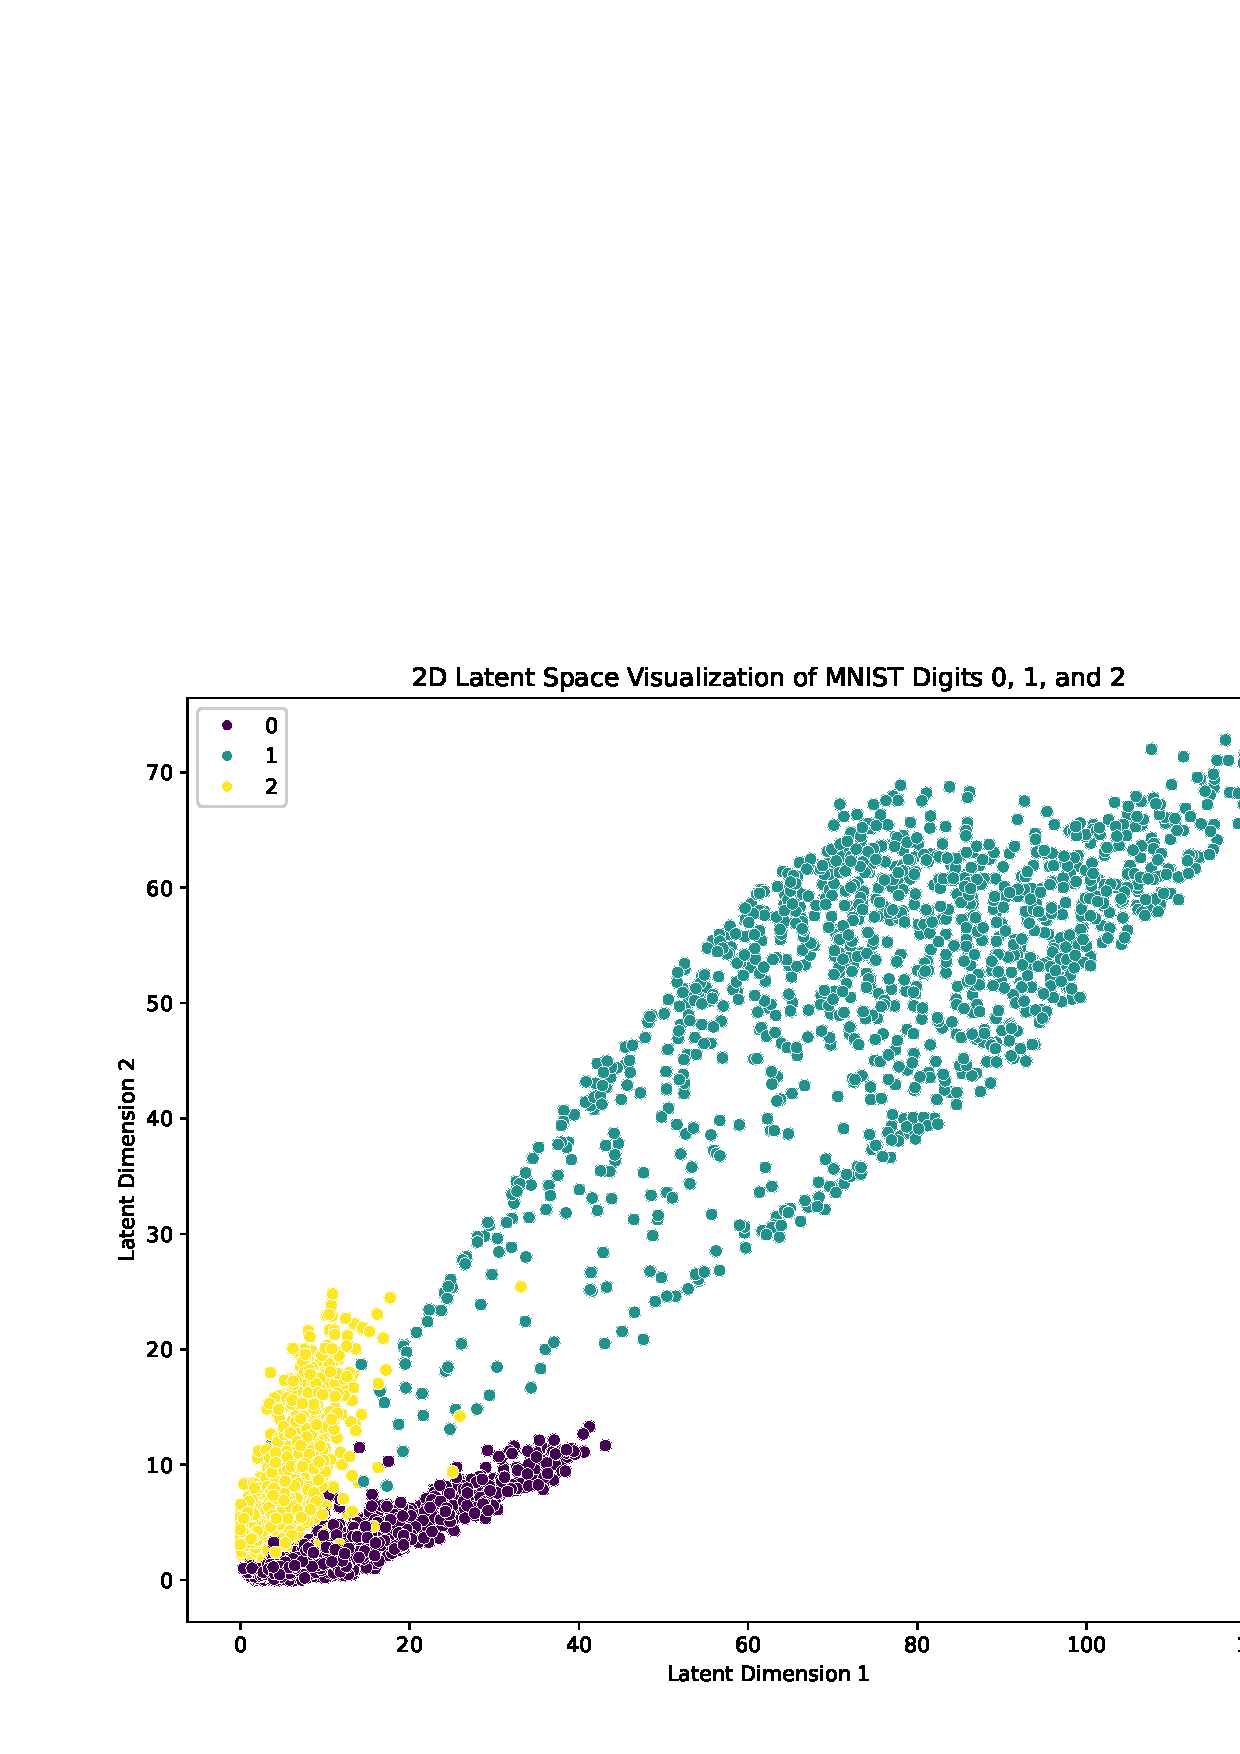
\includegraphics[width=7cm]{image-gen/picture/kaishi6.pdf}
\centering
\caption{MNISTデータセットの0、1、2の潜在空間における分布}
\end{figure}
\subsection{オートエンコーダーの生成}
一般に、画像生成では乱数を入力として処理を行い、画像を生成します。オートエンコーダーにおいては、潜在空間からランダムな値をサンプリングし、それをデコーダーに通すことで画像を生成します。

ここでは、図7の結果を基に、意図的に特定の手書き数字を生成できるかを検証します。ここで生成したい数字を「2」とすると、潜在空間内で「2」に対応するデータは、次元1が0から10、次元2が0から25の範囲内に分布しています。仮に、次元1の値を5、次元2の値を10とする潜在空間上の点を設定し、この点をデコーダーに通して画像を生成します。その結果、図8に示すように、手書き文字の「2」が生成されていることが確認できました。
\begin{figure}[h]
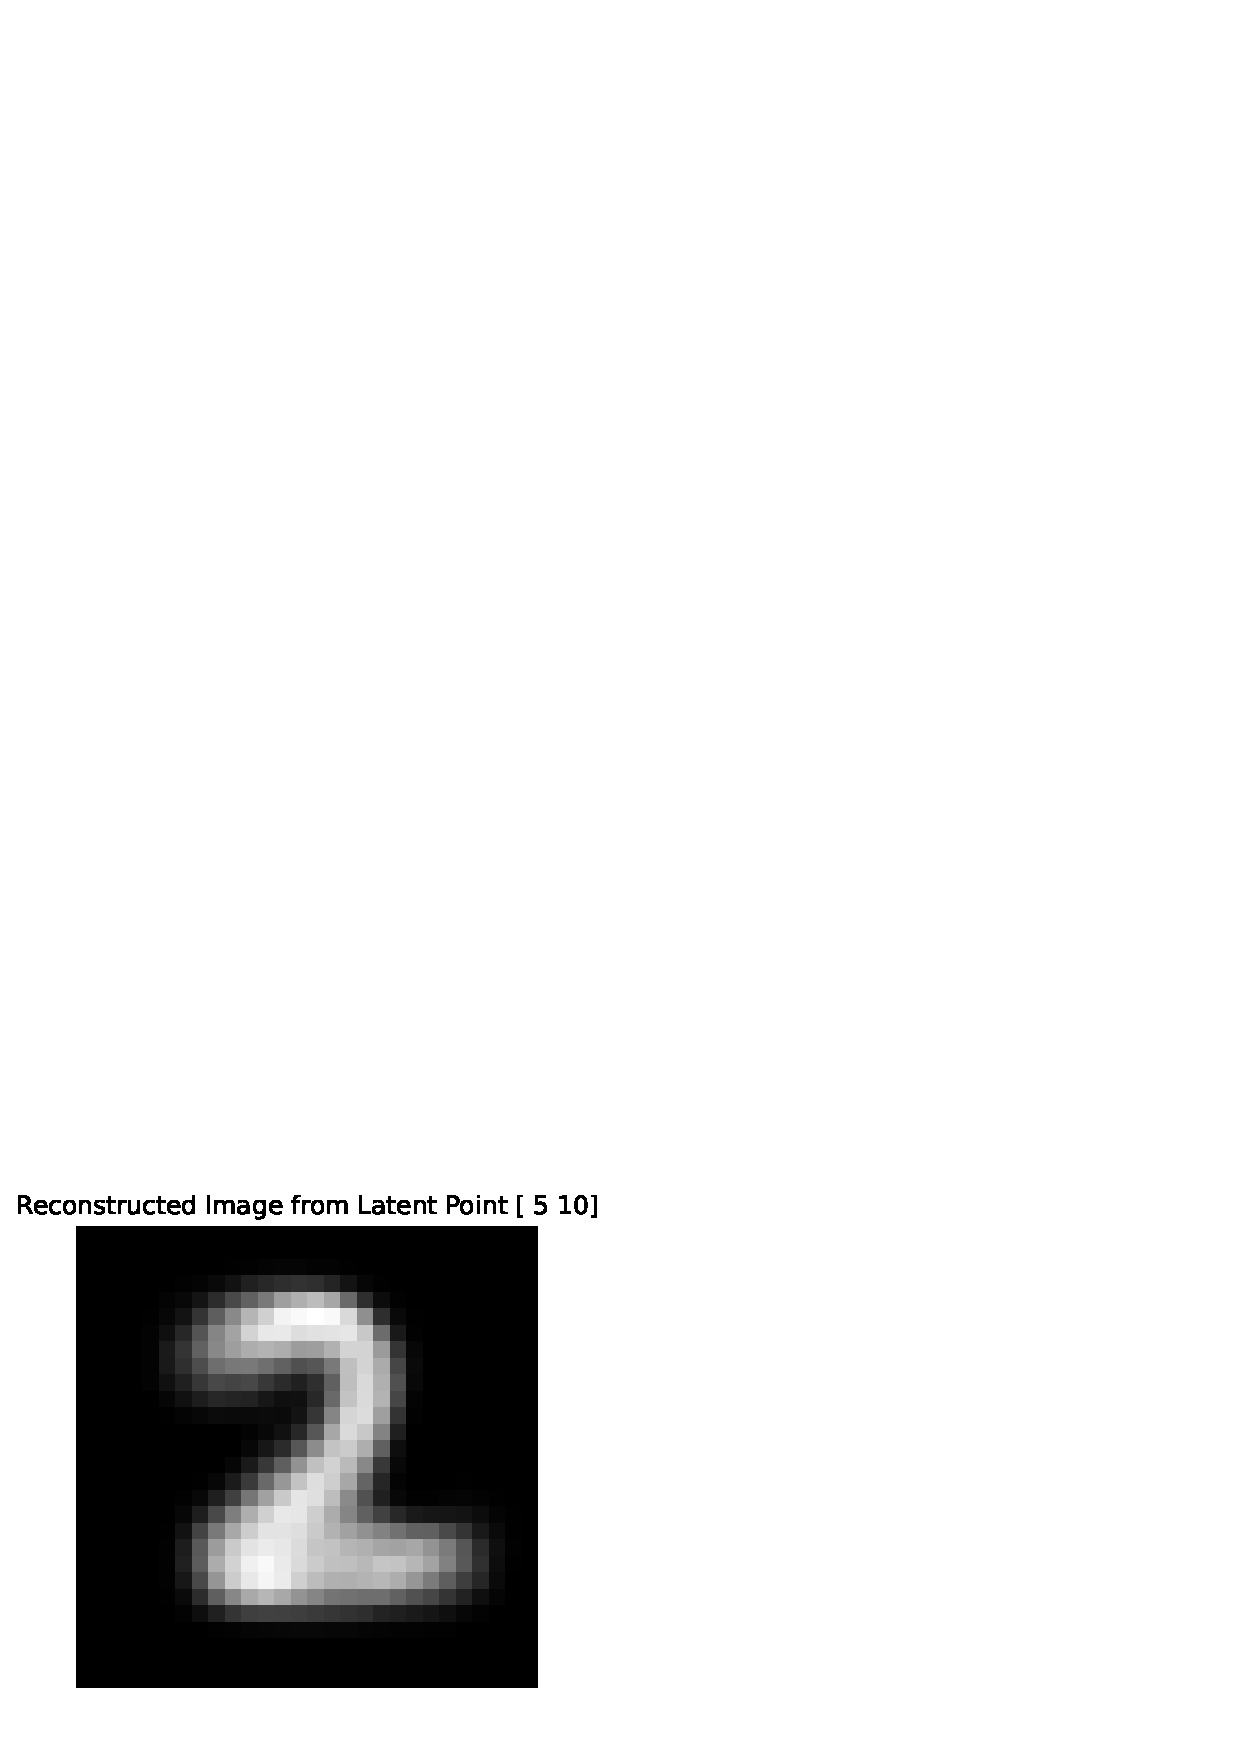
\includegraphics[width=7cm]{image-gen/picture/kaishi7.pdf}
\centering
\caption{潜在空間(5,10)の点から生成した画像}
\end{figure}
\section{ノイズ除去拡散モデル}
\subsection{ノイズ除去拡散モデルの概要}
この節からは、現在の画像生成技術の核となる拡散モデルについて解説します。拡散モデルは、2015年に機械学習および人工知能の研究者であるジャシャ・ソール=ディックスタインによって考案されたもので、非平衡熱力学の概念から着想を得ています。本節では、その中でも特に\textgt{ノイズ除去拡散モデル(Denoising Diffusion Probabilistic Models)}に焦点を当てて紹介します。

ノイズ除去拡散モデルの特徴は、オートエンコーダーのように一度の処理で画像を生成するのではなく、図9のように各ピクセルがランダムな値で構成された砂嵐(ノイズ画像)のような状態から、繰り返しノイズを除去する処理を行い、最終的に高品質な画像を生成する点にあります。
\begin{figure}[h]
\includegraphics[width=13cm]{image-gen/picture/kaishi8.pdf}
\centering
\caption{拡散モデルの画像生成過程例
出典:https://arxiv.org/pdf/2006.11239}
\end{figure}
\subsection{ノイズ除去拡散モデルの学習・画像生成}
まず、ノイズ除去拡散モデルを学習させるためのデータを作成します。ある画像に対して、段階的にわずかなノイズを加えていきます。この操作を繰り返すことで、最終的には各ピクセルが完全にランダムな値で構成された画像に近づいていきます。これは、図10における右から左への処理に対応します。これを\textgt{順方向の拡散過程}と呼びます。

この過程で得られる中間段階の画像と、それぞれの画像に加えられたノイズの情報を学習に利用します。学習の目的は、前述のとおり画像からノイズを除去することです。したがって、ノイズのある画像から加えられたノイズを予測し、その予測値を差し引くことで、ノイズを除去した画像を得ることができます。この処理は、図10における左から右への処理に対応し、画像にノイズを加える過程の逆操作を再現しているといえます。これを\textgt{逆方向の拡散過程}と呼びます。画像生成は、各ピクセルがランダムな値で構成された画像から始まり、前述のノイズ除去処理を繰り返すことで、最終的に高品質な画像が生成されます。
\begin{figure}[h]
\includegraphics[width=10cm]{image-gen/picture/kaishi9.pdf}
\centering
\caption{ノイズの付加と除去の過程 出典:https://arxiv.org/pdf/2006.11239}
\end{figure}
\subsection{ノイズ除去拡散モデルの構造}
それでは、画像に加えられたノイズをどのように予測するのかについて解説します。この問題をより一般的な観点から見ると、入力画像(ノイズを含む画像)と、予測すべき出力(ノイズ)が与えられていることになります。したがって、このタスクの構造は、オートエンコーダーにおける画像の圧縮と復元の過程に類似しています。

異なる点は、予測の対象がオートエンコーダーでは元の画像であるのに対し、ノイズ除去拡散モデルではノイズそのものであるという点です。したがって、基本的な構造はオートエンコーダーと同様に設計することが可能ですが、ノイズ除去拡散モデルでは、より高い精度を実現するために\textgt{U-Net}と呼ばれる構造が用いられます。

U-Netの構造は、オートエンコーダーと同様に、畳み込み処理によって特徴マップを圧縮するエンコーダーと、転置畳み込み処理によって特徴マップを拡大するデコーダーから構成されます。U-Net の特徴的な構造として、\textgt{残差接続}があります。
\begin{figure}[h]
\includegraphics[width=10cm]{image-gen/picture/kaishi10.pdf}
\centering
\caption{U-Netの構造 出典:https://arxiv.org/pdf/1505.04597}
\end{figure}

残差接続とは、図11に示すように、エンコーダー側の各段階で得られる特徴マップを、同じサイズのデコーダー側の特徴マップと積み重ね、その後、図4のように複数種類のフィルタを適用して畳み込み処理を行う構造です。この構造により、エンコーダーの途中で得られた空間的特徴情報がデコーダーに橋渡しされ、画像の位置関係などの情報を保持したまま、より高精度な予測が可能となります。
\section{潜在拡散モデル}
\subsection{潜在拡散モデルの概要}
この節では、イギリスの企業 Stability AI によって一般公開された画像生成モデル Stable Diffusion の中核となる\textgt{潜在拡散モデル(Latent Diffusion Model)}について解説します。Stable Diffusion は 2022 年 10 月に公開され、高価な専用機器を必要とせず一般的なパソコンでも実行できたことから、AI による画像生成が広く普及する契機となりました。

このモデルは、テキストによる指示に従って画像を生成する \textgt{text-to-image モデル}であり、現在一般的に想起される画像生成の代表的な形態です。Stable Diffusion は、ノイズ除去拡散モデルを基盤としつつ、さまざまな改良を加えることで、テキストの指示に忠実で高品質な画像生成を実現しています。

ここでは、その改良点のうち最も精度向上に寄与している\textgt{潜在拡散(Latent Diffusion)}について解説します。潜在拡散モデルでは、オートエンコーダーのように一度画像を圧縮して潜在空間を得た後、その潜在空間上でノイズ除去拡散モデルと同様のノイズ除去処理を行うことで、画像を生成します。
\subsection{潜在拡散モデルの構造・学習・生成}
以前のノイズ除去拡散モデルでは、画像の画素空間(ピクセル空間)上でノイズ除去を行っていたため、高解像度の画像を処理するには膨大な\textgt{計算量}が必要となります。ここでいう計算量とは、画像生成の際に必要となる加算や乗算などの演算回数を指します。計算量を削減しつつ、画像生成の表現力を両立している点が、潜在拡散モデルの大きな特徴です。

具体的には、まずオートエンコーダーと同様に、画像を圧縮および復元するように学習を行います。第3節で紹介したオートエンコーダーでは2次元に圧縮しましたが、潜在拡散モデルでは、より高次元である$32\times32$のような低解像度の特徴マップとして圧縮します。
\begin{figure}[h]
\includegraphics[width=13cm]{image-gen/picture/kaishi11.pdf}
\centering
\caption{潜在拡散モデル 画像:https://arxiv.org/pdf/2112.10752}
\end{figure}

図12に示すように、学習済みのオートエンコーダーに実際の画像を入力し、潜在空間上の特徴マップを得ます。この特徴マップに対して、ノイズ除去拡散モデルと同様に、段階的にノイズを加える処理(順方向の拡散過程)を行います。その後、ノイズが加えられた特徴マップからノイズを予測し、除去するように学習します(逆方向の拡散過程)。

最後に、画像を生成する際には、各ピクセルがランダムな値で構成された特徴マップから始め、前述のノイズ除去処理を繰り返した後、デコーダーを用いて最終的な画像を復元します。
